% Options for packages loaded elsewhere
\PassOptionsToPackage{unicode}{hyperref}
\PassOptionsToPackage{hyphens}{url}
\documentclass[
]{article}
\usepackage{xcolor}
\usepackage{amsmath,amssymb}
\setcounter{secnumdepth}{-\maxdimen} % remove section numbering
\usepackage{iftex}
\ifPDFTeX
  \usepackage[utf8]{inputenc}
  \usepackage[russian]{babel}
  \usepackage[T1]{fontenc}
  \usepackage[utf8]{inputenc}
  \usepackage{textcomp} % provide euro and other symbols
\else % if luatex or xetex
  \usepackage[utf8]{inputenc}
  \usepackage[russian]{babel}
  \usepackage{unicode-math} % this also loads fontspec
  \defaultfontfeatures{Scale=MatchLowercase}
  \defaultfontfeatures[\rmfamily]{Ligatures=TeX,Scale=1}
\fi
\usepackage{lmodern}
\ifPDFTeX\else
  % xetex/luatex font selection
\fi
% Use upquote if available, for straight quotes in verbatim environments
\IfFileExists{upquote.sty}{\usepackage{upquote}}{}
\IfFileExists{microtype.sty}{% use microtype if available
  \usepackage[]{microtype}
  \UseMicrotypeSet[protrusion]{basicmath} % disable protrusion for tt fonts
}{}
\makeatletter
\@ifundefined{KOMAClassName}{% if non-KOMA class
  \IfFileExists{parskip.sty}{%
    \usepackage{parskip}
  }{% else
    \setlength{\parindent}{0pt}
    \setlength{\parskip}{6pt plus 2pt minus 1pt}}
}{% if KOMA class
  \KOMAoptions{parskip=half}}
\makeatother
\usepackage{graphicx}
\makeatletter
\newsavebox\pandoc@box
\newcommand*\pandocbounded[1]{% scales image to fit in text height/width
  \sbox\pandoc@box{#1}%
  \Gscale@div\@tempa{\textheight}{\dimexpr\ht\pandoc@box+\dp\pandoc@box\relax}%
  \Gscale@div\@tempb{\linewidth}{\wd\pandoc@box}%
  \ifdim\@tempb\p@<\@tempa\p@\let\@tempa\@tempb\fi% select the smaller of both
  \ifdim\@tempa\p@<\p@\scalebox{\@tempa}{\usebox\pandoc@box}%
  \else\usebox{\pandoc@box}%
  \fi%
}
% Set default figure placement to htbp
\def\fps@figure{htbp}
\makeatother
\setlength{\emergencystretch}{3em} % prevent overfull lines
\providecommand{\tightlist}{%
  \setlength{\itemsep}{0pt}\setlength{\parskip}{0pt}}
\usepackage{bookmark}
\IfFileExists{xurl.sty}{\usepackage{xurl}}{} % add URL line breaks if available
\urlstyle{same}
\hypersetup{
  pdftitle={отчет},
  hidelinks,
  pdfcreator={LaTeX via pandoc}}

\title{отчет}
\author{}
\date{}

\begin{document}
\maketitle

\section{Цель
работы:}\label{ux446ux435ux43bux44c-ux440ux430ux431ux43eux442ux44b}

Рассчитать и смоделировать движение с обратной связью Меканум-платформы
Kuka Youbot на основе реальных данных, полученных в ходе лабораторных
работ №1-3.

\section{Темы лабораторных
работ:}\label{ux442ux435ux43cux44b-ux43bux430ux431ux43eux440ux430ux442ux43eux440ux43dux44bux445-ux440ux430ux431ux43eux442}

\begin{itemize}
\tightlist
\item
  Лабораторная работа №1: поступательное движение тележки робота по
  заданной траектории.
\item
  Лабораторная работа №2: вращательное движение тележки робота с
  заданной угловой скоростью.
\item
  Лабораторная работа №3: сложное движение тележки робота по заданной
  траектории.
\end{itemize}

\section{Содержание
отчета:}\label{ux441ux43eux434ux435ux440ux436ux430ux43dux438ux435-ux43eux442ux447ux435ux442ux430}

\begin{itemize}
\tightlist
\item
  Описание алгоритма моделирования движения с обратной связью
\item
  Графики идеальной, экспериментальной и полученной с использованием
  алгоритма обратной связи траекторий, скоростей в ССК и НСК
\item
  Численные расчеты расхождения движения с обратной связью относительно
  идеальных данных, их сравнение с аналогичными данными, полученными из
  экспериментальных данных
\end{itemize}

\section{Алгоритм моделирования движения с обратной
связью}\label{ux430ux43bux433ux43eux440ux438ux442ux43c-ux43cux43eux434ux435ux43bux438ux440ux43eux432ux430ux43dux438ux44f-ux434ux432ux438ux436ux435ux43dux438ux44f-ux441-ux43eux431ux440ux430ux442ux43dux43eux439-ux441ux432ux44fux437ux44cux44e}

\begin{enumerate}
\tightlist
\item
  Сформировать вектор ошибок движения:{}где {} - вектор скоростей в
  связанной системе координат платформы
\item
  Рассчитать паразитные ускорения:{}
\item
  Введем вектора скорректированных скоростей {}, смоделированных на них
  реальных скоростей ({}), предполагая те же паразитные ускорения, что и
  в алгоритме, и координаты {}, основанных на {} для первых двух
  итераций алгоритма:\\
  {}\strut \\
  {}\strut \\
  {}\strut \\
  {} {}{}где {} -коэффициент обратной связи по скоростям, {} -
  коэффициент обратной связи по координатам
\item
  Дальнейшие итерации алгоритма:\\
  {}{}{}{} - матрица поворота, необходимая для переноса векторов между
  НСК и ССК:
\end{enumerate}

{}

В дальнейших расчетах будут использоваться следующие значения
коэффициентов обратной связи:\\
{}\strut \\
{}

\section{Лабораторная работа
№1}\label{ux43bux430ux431ux43eux440ux430ux442ux43eux440ux43dux430ux44f-ux440ux430ux431ux43eux442ux430-1}

\subsection{Графики}\label{ux433ux440ux430ux444ux438ux43aux438}

\pandocbounded{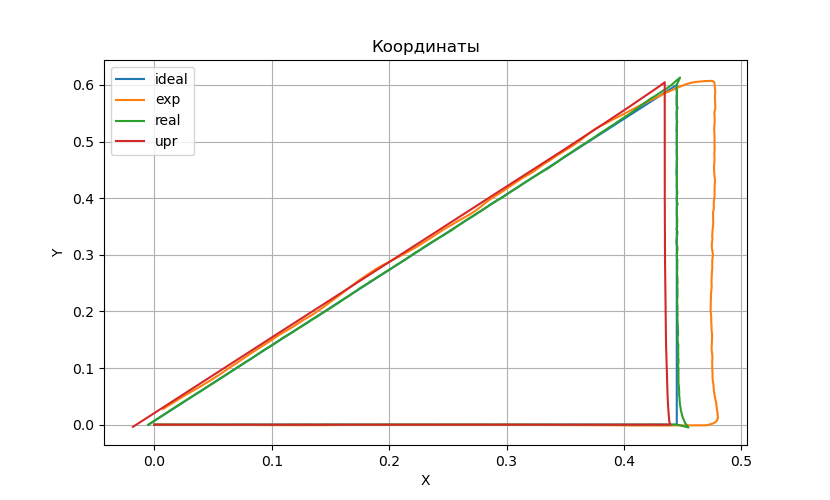
\includegraphics[keepaspectratio]{/temp/lab1_Координаты.png}}

\pandocbounded{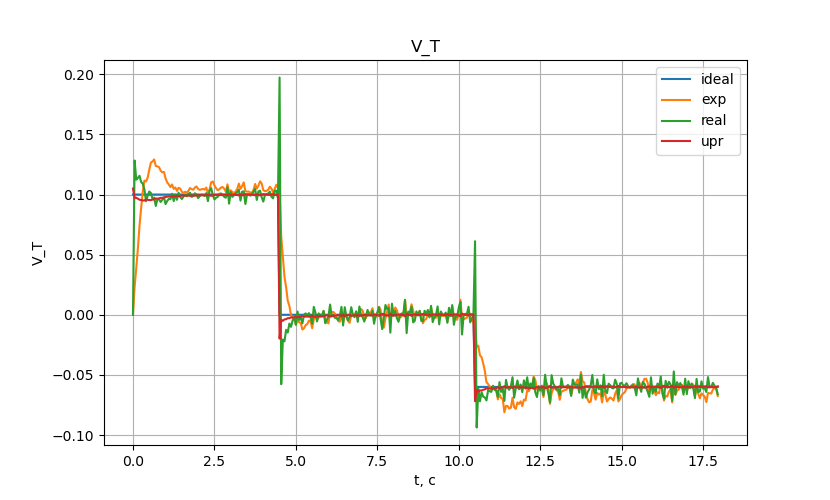
\includegraphics[keepaspectratio]{/temp/lab1_V_T.png}}

\pandocbounded{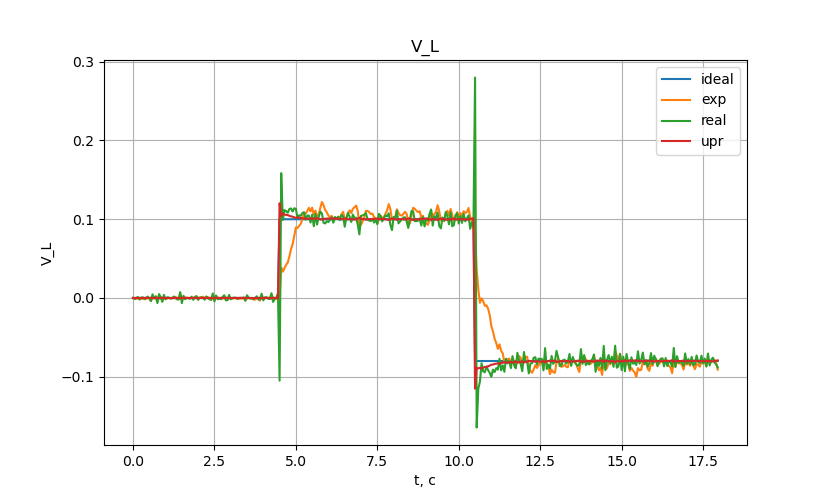
\includegraphics[keepaspectratio]{/temp/lab1_V_L.png}}

\pandocbounded{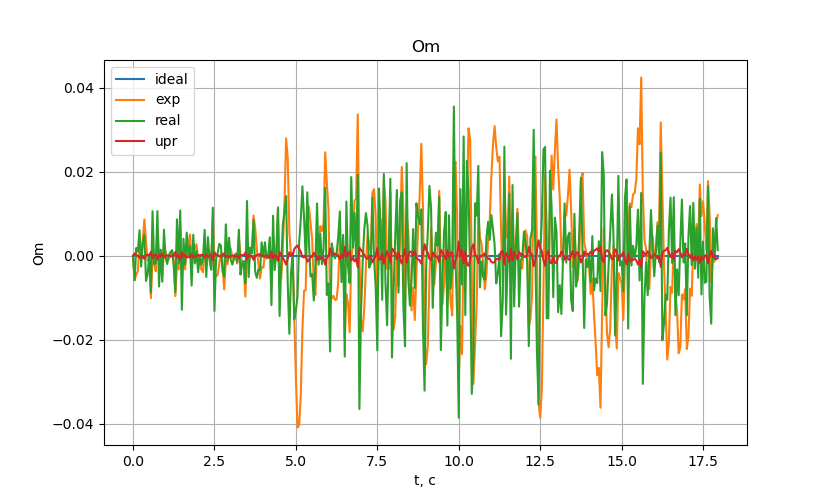
\includegraphics[keepaspectratio]{/temp/lab1_Om.png}}

\pandocbounded{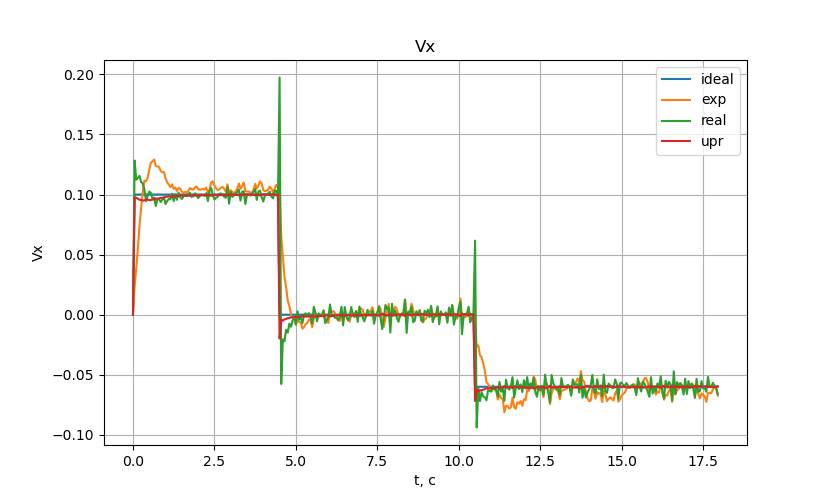
\includegraphics[keepaspectratio]{/temp/lab1_Vx.png}}

\pandocbounded{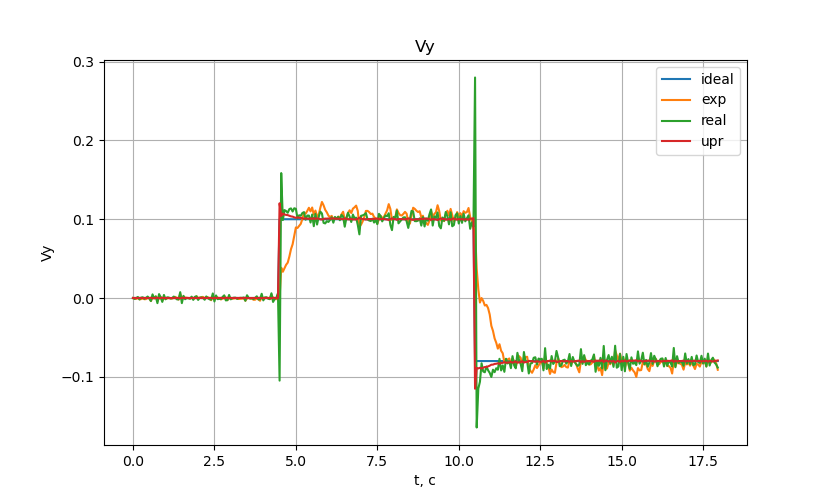
\includegraphics[keepaspectratio]{/temp/lab1_Vy.png}}

\subsection{Среднеквадратичные
отклонения}\label{ux441ux440ux435ux434ux43dux435ux43aux432ux430ux434ux440ux430ux442ux438ux447ux43dux44bux435-ux43eux442ux43aux43bux43eux43dux435ux43dux438ux44f}

Отклонение идеальной траектории от экспериментальной по оси X:
0.001357м\\
Отклонение идеальной траектории от скорректированной по оси X:
0.000076м\\
Отклонение идеальной траектории от экспериментальной по оси Y:
0.001521м\\
Отклонение идеальной траектории от скорректированной по оси Y:
0.000109м\\
Отклонение идеальной траектории от экспериментальной по углу поворота
{}: 0.000260рад\\
Отклонение идеальной траектории от скорректированной по углу поворота
{}: 0.000032рад\\
Отклонение идеальной {} от экспериментальной: 0.000720м/с\\
Отклонение идеальной {} от скорректированной: 0.000804м/с\\
Отклонение идеальной {} от экспериментальной: 0.001037м/с\\
Отклонение идеальной {} от скорректированной: 0.001270м/с\\
Отклонение идеальной {} от экспериментальной: 0.000689рад/с\\
Отклонение идеальной {} от скорректированной: 0.000601рад/с

\section{Лабораторная работа
№2}\label{ux43bux430ux431ux43eux440ux430ux442ux43eux440ux43dux430ux44f-ux440ux430ux431ux43eux442ux430-2}

\subsection{Графики}\label{ux433ux440ux430ux444ux438ux43aux438-1}

\pandocbounded{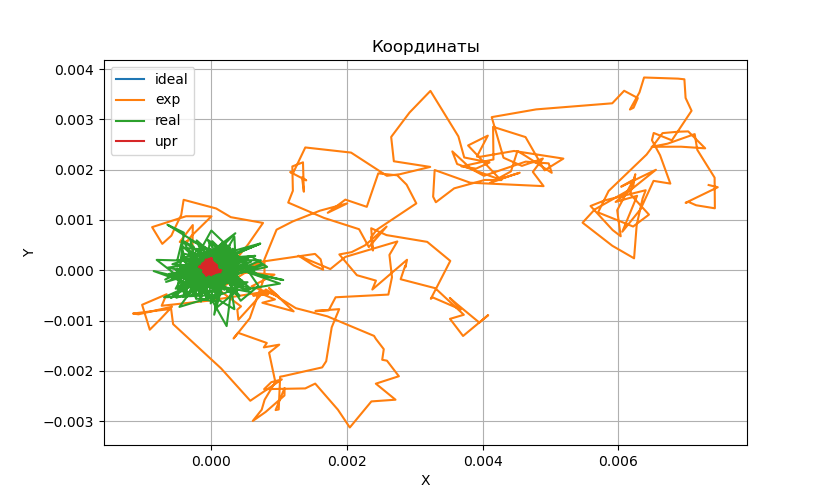
\includegraphics[keepaspectratio]{/temp/lab2_Координаты.png}}

\pandocbounded{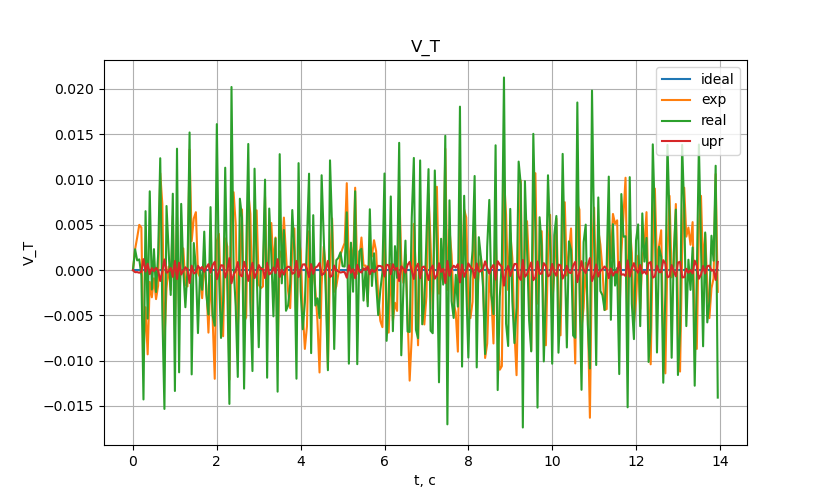
\includegraphics[keepaspectratio]{/temp/lab2_V_T.png}}

\pandocbounded{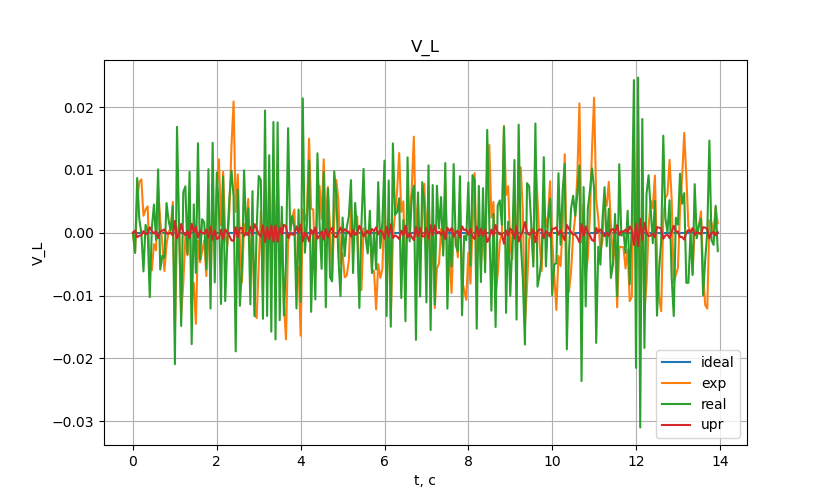
\includegraphics[keepaspectratio]{/temp/lab2_V_L.png}}

\pandocbounded{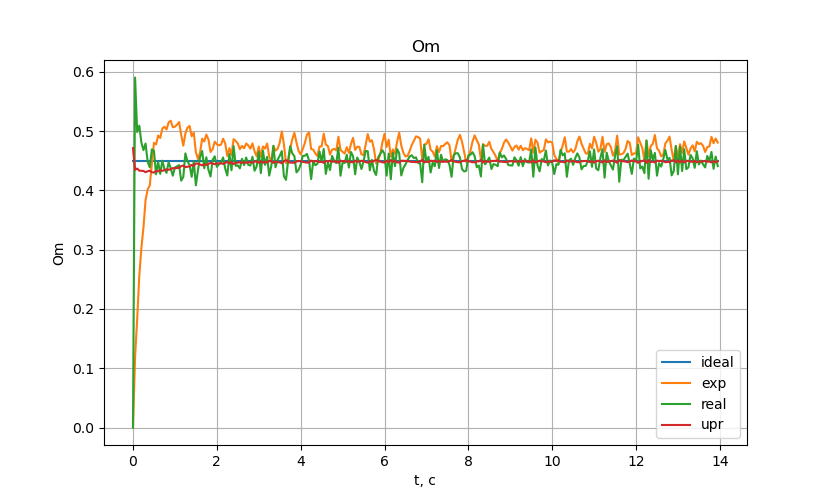
\includegraphics[keepaspectratio]{/temp/lab2_Om.png}}

\pandocbounded{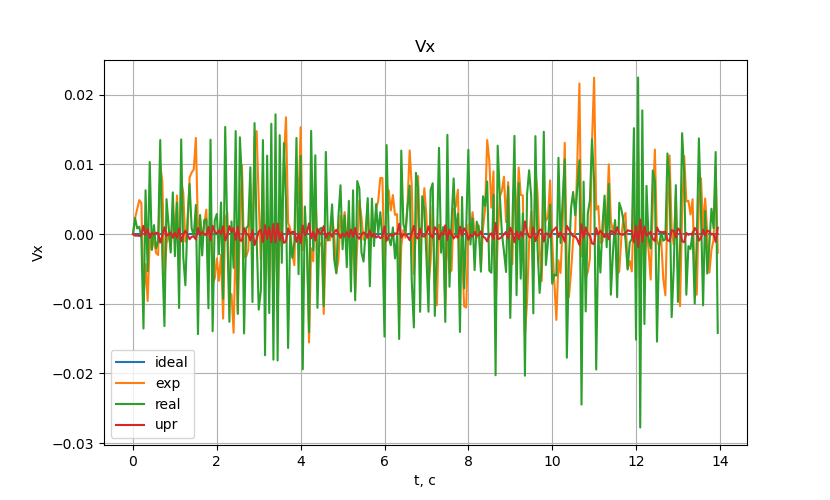
\includegraphics[keepaspectratio]{/temp/lab2_Vx.png}}

\pandocbounded{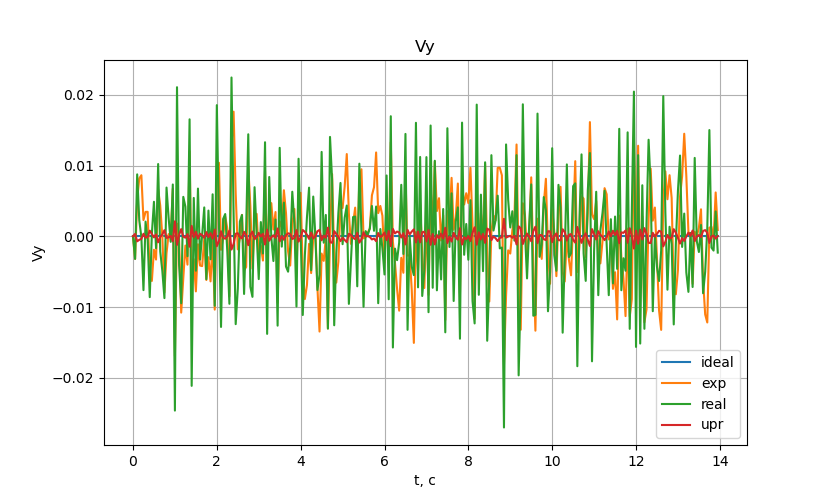
\includegraphics[keepaspectratio]{/temp/lab2_Vy.png}}

\subsection{Среднеквадратичные
отклонения}\label{ux441ux440ux435ux434ux43dux435ux43aux432ux430ux434ux440ux430ux442ux438ux447ux43dux44bux435-ux43eux442ux43aux43bux43eux43dux435ux43dux438ux44f-1}

Отклонение идеальной траектории от экспериментальной по оси X:
0.000223м\\
Отклонение идеальной траектории от скорректированной по оси X:
0.000020м\\
Отклонение идеальной траектории от экспериментальной по оси Y:
0.000103м\\
Отклонение идеальной траектории от скорректированной по оси Y:
0.000019м\\
Отклонение идеальной траектории от экспериментальной по углу поворота
{}: 0.009310рад\\
Отклонение идеальной траектории от скорректированной по углу поворота
{}: 0.000278рад\\
Отклонение идеальной {} от экспериментальной: 0.000332м/с\\
Отклонение идеальной {} от скорректированной: 0.000490м/с\\
Отклонение идеальной {} от экспериментальной: 0.000432м/с\\
Отклонение идеальной {} от скорректированной: 0.000594м/с\\
Отклонение идеальной {} от экспериментальной: 0.002967рад/с\\
Отклонение идеальной {} от скорректированной: 0.001965рад/с

\section{Лабораторная работа
№3}\label{ux43bux430ux431ux43eux440ux430ux442ux43eux440ux43dux430ux44f-ux440ux430ux431ux43eux442ux430-3}

\subsection{Графики}\label{ux433ux440ux430ux444ux438ux43aux438-2}

\pandocbounded{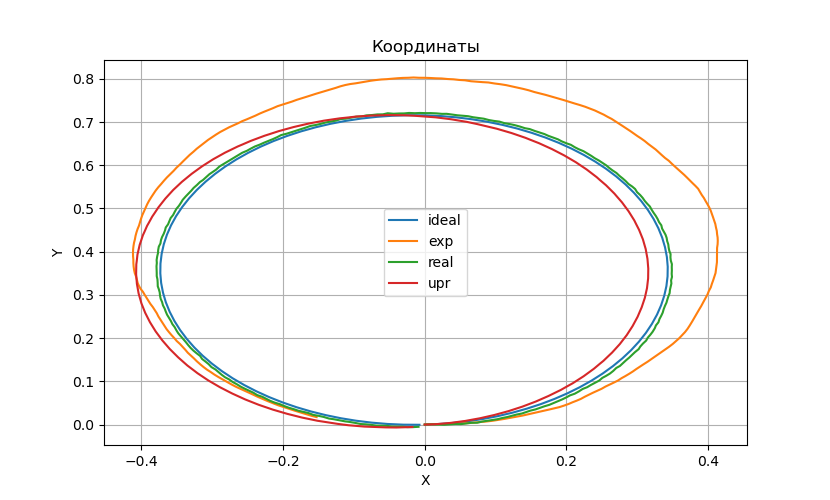
\includegraphics[keepaspectratio]{/temp/lab3_Координаты.png}}

\pandocbounded{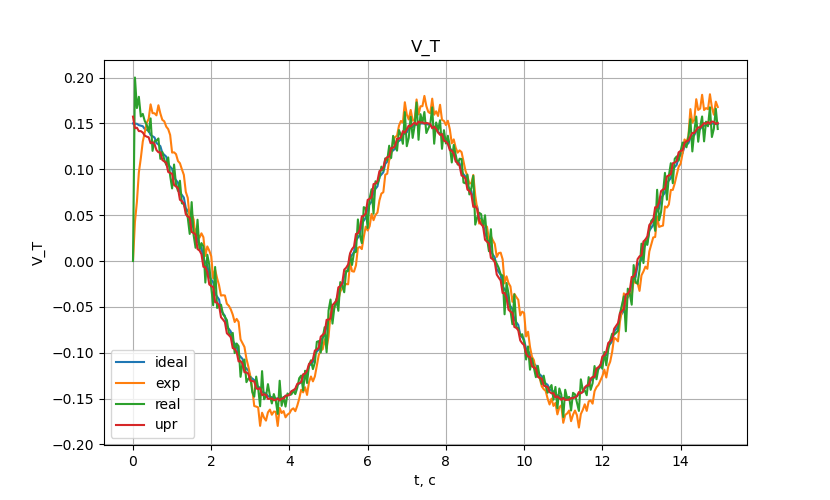
\includegraphics[keepaspectratio]{/temp/lab3_V_T.png}}

\pandocbounded{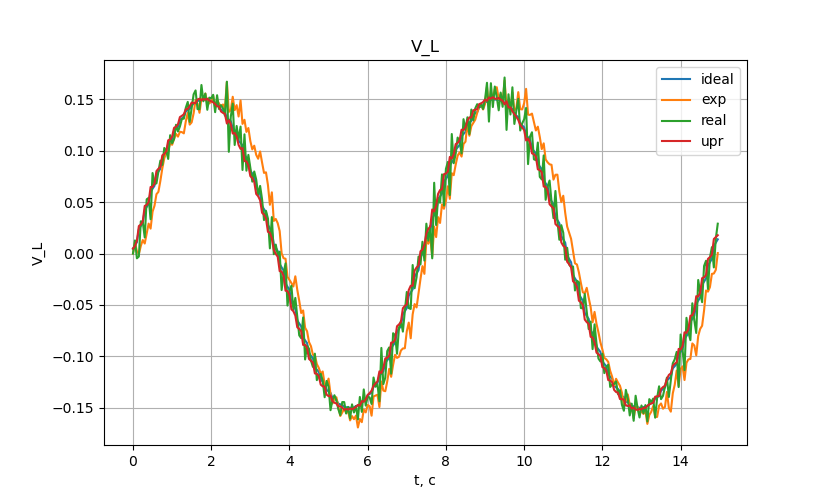
\includegraphics[keepaspectratio]{/temp/lab3_V_L.png}}

\pandocbounded{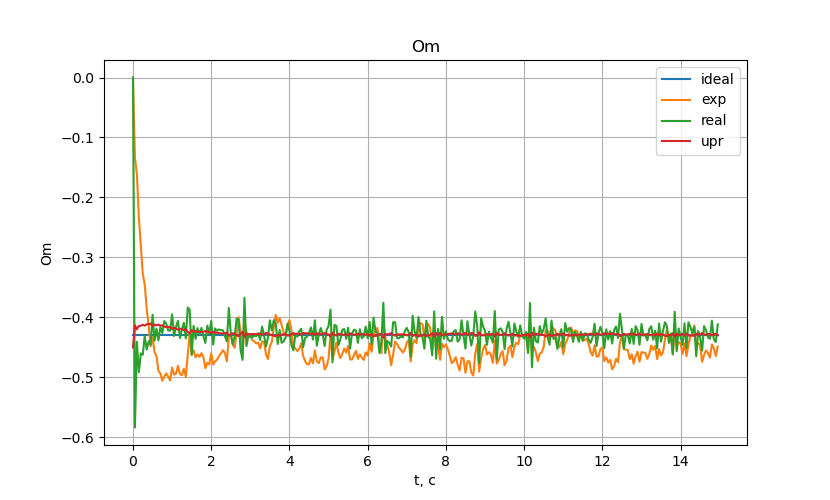
\includegraphics[keepaspectratio]{/temp/lab3_Om.png}}

\pandocbounded{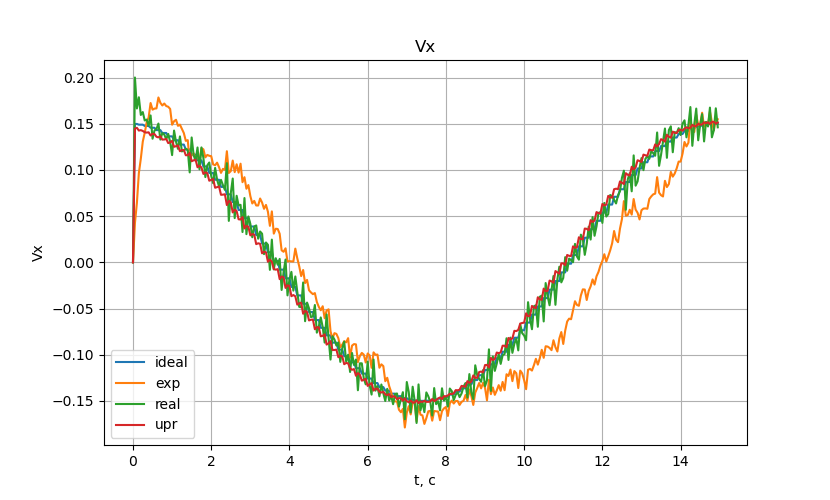
\includegraphics[keepaspectratio]{/temp/lab3_Vx.png}}

\pandocbounded{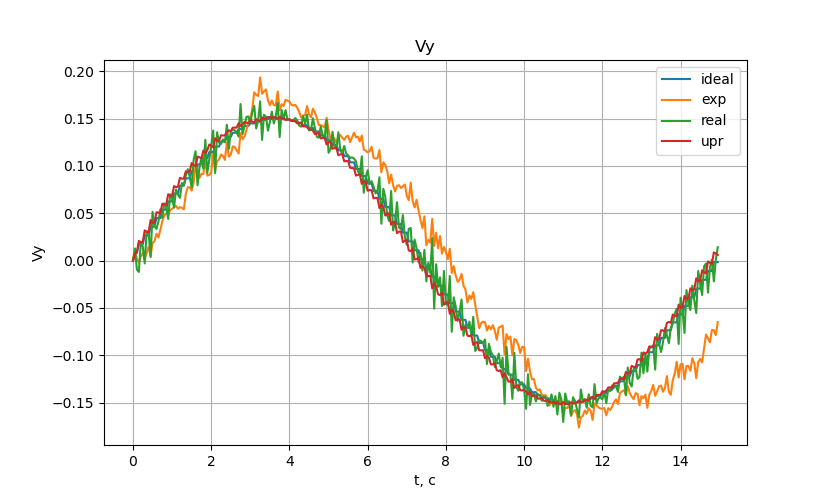
\includegraphics[keepaspectratio]{/temp/lab3_Vy.png}}

\subsection{Среднеквадратичные
отклонения}\label{ux441ux440ux435ux434ux43dux435ux43aux432ux430ux434ux440ux430ux442ux438ux447ux43dux44bux435-ux43eux442ux43aux43bux43eux43dux435ux43dux438ux44f-2}

Отклонение идеальной траектории от экспериментальной по оси X:
0.004975м\\
Отклонение идеальной траектории от скорректированной по оси X:
0.000266м\\
Отклонение идеальной траектории от экспериментальной по оси Y:
0.005547м\\
Отклонение идеальной траектории от скорректированной по оси Y:
0.000220м\\
Отклонение идеальной траектории от экспериментальной по углу поворота
{}: 0.009409рад\\
Отклонение идеальной траектории от скорректированной по углу поворота
{}: 0.000254рад\\
Отклонение идеальной {} от экспериментальной: 0.001326м/с\\
Отклонение идеальной {} от скорректированной: 0.000899м/с\\
Отклонение идеальной {} от экспериментальной: 0.001163м/с\\
Отклонение идеальной {} от скорректированной: 0.000759м/с\\
Отклонение идеальной {} от экспериментальной: 0.002854рад/с\\
Отклонение идеальной {} от скорректированной: 0.001923рад/с

\section{Выводы}\label{ux432ux44bux432ux43eux434ux44b}

Добавление обратной связи на порядок уменьшил отклонение траектории от
идеальной; также значительно уменьшил отклонения по скоростям.

\end{document}
